\chapter{Quantifying the Effects of Hydrogen Bonding on Nitrile Frequencies in GFP: Beyond Solvent Exposure}\label{gfp-hbond}

%Vibrational spectroscopy is a powerful tool for characterizing the complex non-covalent interactions that arise in biological systems.
%The nitrile stretching frequency has proven to be a particularly convenient biological probe, but the interpretation of the spectra of nitriles is complicated by their sensitivity to local hydrogen bonding interactions.
%This often inhibits the straightforward interpretation of nitrile spectra by requiring knowledge of the molecular level details of the local environment surrounding the nitrile.
%While the effect of hydrogen bonds on nitrile frequencies has been well documented for small nitriles in solution, there have been relatively few studies of these effects in a complex protein system.
%Therefore, we introduced a nitrile probe at nine locations throughout green fluorescent protein (GFP) and compared the mean vibrational frequency of each probe to the specific hydrogen bonding geometries observed in molecular dynamics (MD) simulations.
%We show that a continuum of hydrogen bonding angles is found depending on the particular location of each nitrile, and that the differences in these angles account for the differences in the measured nitrile frequency.
%We further observed that the temperature dependence of the nitrile frequencies (measured as a frequency-temperature line slope, FTLS) was a good indicator of the hydrogen bonding interactions of the probe, even in scenarios where the nitrile was involved in complex and restricted hydrogen bonds, both from protein and from water.
%While constant offsets to the nitrile frequency to all hydrogen bonding environments have been applied before to interpret shifts in nitrile frequency, we show that this is insufficient in systems where the hydrogen bonds may be restricted by the surrounding medium.
%However, the strength of the observed correlation between nitrile frequency and hydrogen bonding angle suggests that it may be possible to disentangle electrostatic effects and effects of the orientation of hydrogen bonding on the nitrile stretching frequency.
%Meanwhile, the experimental measurement of the FTLS of the nitrile is an excellent tool to identify changes in the hydrogen bonding interactions for a particular probe.

%%%%%%%%%%%%%%%%%%%%%%%%%%%%%%%%%%%%%%%%%%%%%%%%%%%%%%%%%%%%%%%%
%%%%%%%%%%%%%%%%%%%%%%%%%%%%%%%%%%%%%%%%%%%%%%%%%%%%%%%%%%%%%%%%
\section{Publication note} \label{hbond-pub-note}
%%%%%%%%%%%%%%%%%%%%%%%%%%%%%%%%%%%%%%%%%%%%%%%%%%%%%%%%%%%%%%%%
%%%%%%%%%%%%%%%%%%%%%%%%%%%%%%%%%%%%%%%%%%%%%%%%%%%%%%%%%%%%%%%%

Portions of this chapter are adapted from the following publication: 

\noindent Jeremy T. First, Joshua D. Slocum, Lauren J. Webb; Quantifying the Effects of Hydrogen Bonding on Nitrile Frequencies in GFP: Beyond Solvent Exposure. \emph{Journal of Physical Chemistry B}. \textbf{2018}, \emph{122}, 6735-6743.

JTF performed all calculations.
All code, force field parameters, structures, and other starting files used for the simulation, analysis, processing of data, and figure generation can be accessed at:
\url{https://github.com/jeremyfirst22/GFP_HBond}. 
JDS performed all experiments. The experimental methods are ommited from this Chapter, but they may be found in the publication.

%%%%%%%%%%%%%%%%%%%%%%%%%%%%%%%%%%%%%%%%%%%%%%%%%%%%%%%%%%%%%%%%
%%%%%%%%%%%%%%%%%%%%%%%%%%%%%%%%%%%%%%%%%%%%%%%%%%%%%%%%%%%%%%%%
\section{Introduction}\index{hbond-intro}
%%%%%%%%%%%%%%%%%%%%%%%%%%%%%%%%%%%%%%%%%%%%%%%%%%%%%%%%%%%%%%%%
%%%%%%%%%%%%%%%%%%%%%%%%%%%%%%%%%%%%%%%%%%%%%%%%%%%%%%%%%%%%%%%%

The complex networks of non-covalent interactions that arise from the arrangement of thousands of partially charged atoms in biological molecules are responsible for many important biomolecular functions, including protein folding, protein-protein interactions, membrane fluidity and permeation, ligand binding, signaling pathways, and catalysis \cite{Honig1995}.
Characterizing and understanding the molecular details of the environments that give rise to biological function is of critical importance to modern biophysics.
The inherent spatial and temporal resolution of molecular vibrations have been exploited by many researchers to directly probe biological systems.
Specifically, the nitrile stretching frequency has been widely used as a probe of site-specific dynamics \cite{Fang2008, Sigala2007, Yoshikawa1985}, hydration \cite{Waegele2009, Oh2008}, and electric fields\cite{Webb2008, Slocum2016, Shrestha2015, Shrestha2017, Andrews2000, Andrews2002} in a variety of biological systems due to its extraordinary environmental sensitivity.
Nitrile vibrational probes absorb in a relatively transparent region of the infrared spectrum, have reasonable oscillator strengths \cite{Webb2008}, and can be easily incorporated through a variety of synthetic and biosynthetic methods\cite{Fafarman2006, Getahun2003, Kirshenbaum2002} to interrogate DNA, proteins, and membranes. 

Despite the widespread use of nitriles as biomolecular probes and the relative ease with which their frequencies can be measured in a variety of applications, it is not trivial to meaningfully interpret a measured nitrile frequency in a complex biological system.
This is largely due to the convolution of the competing effects of Coulombic frequency shifts, commonly referred to as the vibrational Stark effect (VSE), and frequency shifts due to specific interactions such as hydrogen bonding.
While the effects of solvent electric field and specific hydrogen bonding interactions on nitrile frequencies have been well characterized for small nitriles in solution \cite{Levinson2012, Blasiak2017, Deb2016}, the theoretical basis for these convoluted effects does not always successfully translate to the interpretation of nitrile frequencies in more complex systems like a solvated protein.
Indeed, the ability to interpret nitrile frequencies in terms of electric fields via a VSE analysis when the nitrile experiences hydrogen bonds has been under question for quite some time \cite{Slocum2016, Fafarman2010, Bagchi2012, Slocum2018}.
While it is clear that VSE analyses of nitrile frequencies can be used to quantify relative electric fields between nitriles that are engaged in similar hydrogen bonding interactions \cite{Slocum2016}, there is still debate on how to define criteria that must be met in order for two nitriles to be classified within this regime.
This is further complicated by a lack of experimental methodologies to specifically test \emph{in situ} if these hydrogen bonding criteria are met.
Conversely, the use of nitrile frequencies as site-specific probes of solvent exposure inherently ignores any electrostatic contribution to the frequency by equating blue shifted spectra with solvent exposed locations and red shifted spectra with buried locations.
The possibility that electric field effects would red-shift the spectrum of a solvent exposed nitrile or blue-shift the spectrum of a buried nitrile is usually not considered.

Significant theoretical effort has been made towards developing quantitative models that can capture the competing effects of hydrogen bonding and Coulombic forces on nitrile frequencies.
Early theories focused on relating bulk properties of the solvent to the nitrile frequency \cite{Kirkwood1934, Onsager1936}.
While these theories have worked well for aprotic solvents, it has become increasingly apparent that specific molecular interactions between the nitrile and the surrounding solvent are a major contributor to the nitrile frequency in environments rich in hydrogen bond donors, such as aqueous solvent or a protein interior \cite{Blasiak2017}.
Recently, B\l{}asiak et al. developed a highly quantitative model based on combined quantum mechanical (QM) methods and molecular dynamics (MD) simulations that accurately captured the direction of nitrile frequency shifts in different solvent environments \cite{Blasiak2016}.
However, these models are computationally expensive and it is therefore useful to develop a nitrile classification system based strictly on geometric parameters of hydrogen bonding interactions that can be determined from MD simulations as a complement to rigorous QM modeling.


Using \emph{ab initio} calculations of clusters of water hydrogen bound to both acetonitrile and methyl thiocyanate, Choi et al. observed that in linear $\sigma$-hydrogen bonds the nitrile bond was shortened, leading to an increase in the nitrile stretching frequency.
However, at the small angles found in $\pi$-hydrogen bonds, the nitrile bond was lengthened leading to a decrease in electron density and a decrease in the nitrile frequency \cite{Choi2008}.
Fafarman et al. showed that vibrational frequencies of nitriles involved in unrestricted hydrogen bonds can be deconvoluted into electrostatic effects and hydrogen bonding effects by comparing nitrile frequencies to an independent $^{13}$C NMR parameter \cite{Fafarman2010}.
For nitriles that were well exposed to water, the authors observed a constant vibrational absorption shift of 10 \si{\wn} relative to the observed NMR chemical shift, which was in good agreement with the calculated frequencies for linear hydrogen bonds.
However, in the confined environment of the interior of a protein, steric interactions often enforce non-linear hydrogen bonding geometries.
While these issues have been examined theoretically, there has not been an experimental study on the effects of hydrogen bonding on nitrile frequencies in such cases.

Our laboratory has been particularly interested in experiments that can disentangle the contributions of hydrogen bonding from other influences on the nitrile vibrational frequency, such as those from the VSE.
Measurement of the temperature dependence of the nitrile absorption frequency has been useful in this regard.
In 2003, Getahun et al. first reported the linear temperature dependence of the nitrile stretching frequencies of nitrile-substituted amino acids, with anomalous narrowing of the absorption spectrum with increasing temperature \cite{Getahun2003}.
This observation inspired the use of the nitrile as a probe in conformational or unfolding studies initiated with a temperature jump \cite{Getahun2003, Huang2003}.
In 2007, Maienschein-Cline and Londergan used the temperature dependence of the nitrile frequency to demonstrate that the nitriles were also probes of local hydrogen bonding and solvent dynamics \cite{Maienschein-Cline2007}.
In 2012, Fafarman and Boxer used the temperature dependence of a nitrile to distinguish between two subpopulations of the spectrum of a nitrile in a protein \cite{Fafarman2010a}.
Finally, in 2015, Adhikary et al. postulated that the temperature dependence of the nitrile absorption measured via the frequency-temperature line slope (FTLS) was related to the hydrogen bonding environment experienced by small nitriles in various solvents and in proteins, and the authors were able to use the nitrile FTLS to assess whether or not a particular location was buried or solvent exposed \cite{Adhikary2015}.

While nitrile frequencies have clearly been useful in determining site-specific solvent exposure in proteins, it is often overlooked that solvent exposure is not a binary state, in which the nitrile is either solvent exposed or buried.
While locations on a protein surface might have a relatively constant extent of solvation, locations within a protein can experience a near continuous range of solvent exposure depending on microscopic details of the steric and electrostatic landscape at any given location in the protein's 3D structure.
Moreover, the hydrogen bond strength and geometry may change continuously based on the dynamics of the protein and the solvent.
In this study, we examine these effects using green fluorescent protein (GFP) as a model system.
The water filled \textbeta{}-barrel of GFP provides a range of different hydrogen bonding profiles because the complex network of confined water on the interior of the protein is stabilized by hydrogen bonds to other waters and nearby protein residues and varies in allowed hydrogen bonding geometries, rates of diffusion, and interaction strength.
Each of these different hydrogen bonding environments could contribute to a frequency shift of differing magnitude in a way not described by the VSE.
Here, we use a combination of FTLS measurements and MD simulations to show that the FTLS is related to small differences in hydrogen bonding profiles and is therefore useful beyond just the Boolean classification of a nitrile as either engaging in hydrogen bonding or free from hydrogen bonding.
Instead, the FTLS can be used to differentiate a range of solvent exposure and even differences in specific hydrogen bonding angles.
This makes the FTLS a powerful diagnostic tool for interpreting any nitrile spectrum, as it allows for the rapid comparison of hydrogen bonding interactions of different states.
In the context of a VSE experiment, the FTLS could confirm that the hydrogen bonding interactions have not changed from the reference to perturbed state. 

To evaluate the FTLS of nitriles as a diagnostic tool of hydrogen bonding environment, we biosynthetically incorporated \emph{p}-cyanophenylalanine (CNF) at nine locations in GFP.
The locations were chosen based on the PDB crystal structure 2b3p\cite{Pedelacq2006} to sample a broad range of solvent accessibility and hydrogen bonding environments.
Using the crystal structure, we classified \emph{a priori} the locations as solvent exposed or buried based on the crude assessment of whether or not the side chain was pointed into the interior of the \textbeta{}-barrel.
The nine locations chosen are shown in Figure \ref{fig:hbond-system}, where the colored spheres indicate a residue that was independently mutated to CNF.
We collected temperature dependent Fourier transform infrared (FTIR) spectra and performed MD simulations of each nitrile-containing protein variant.
We found that there is a strong correlation between the FTLS and the solvent accessible surface area (SASA) of the CNF residue (determined from MD simulations) despite the diverse hydrogen bonding profiles.
This indicates that the FTLS can be used reliably and rapidly to test differences in hydrogen bonding interactions of nitrile probes.
Additionally, we compared the measured stretching frequencies of nitriles involved in various restricted hydrogen bonding orientations (again determined from MD simulations) to the effects predicted by changes in the angle of the hydrogen bond to the nitrile.
We found that the observed vibrational shifts of the nitrile in each location can be attributed almost entirely to the average orientation of hydrogen bonds experienced by the nitrile.
Although acetonitrile and CNF are structurally different, we expect them to behave similarly in this regard, as they have been shown to respond similarly to other spectroscopic perturbations \cite{Getahun2003}.
This observation confirms the predictions by Choi et al. and underlines the importance of understanding the molecular-level details of the hydrogen bonding interactions to the nitrile  before interpreting its vibrational spectrum.

\begin{figure}
    \center
    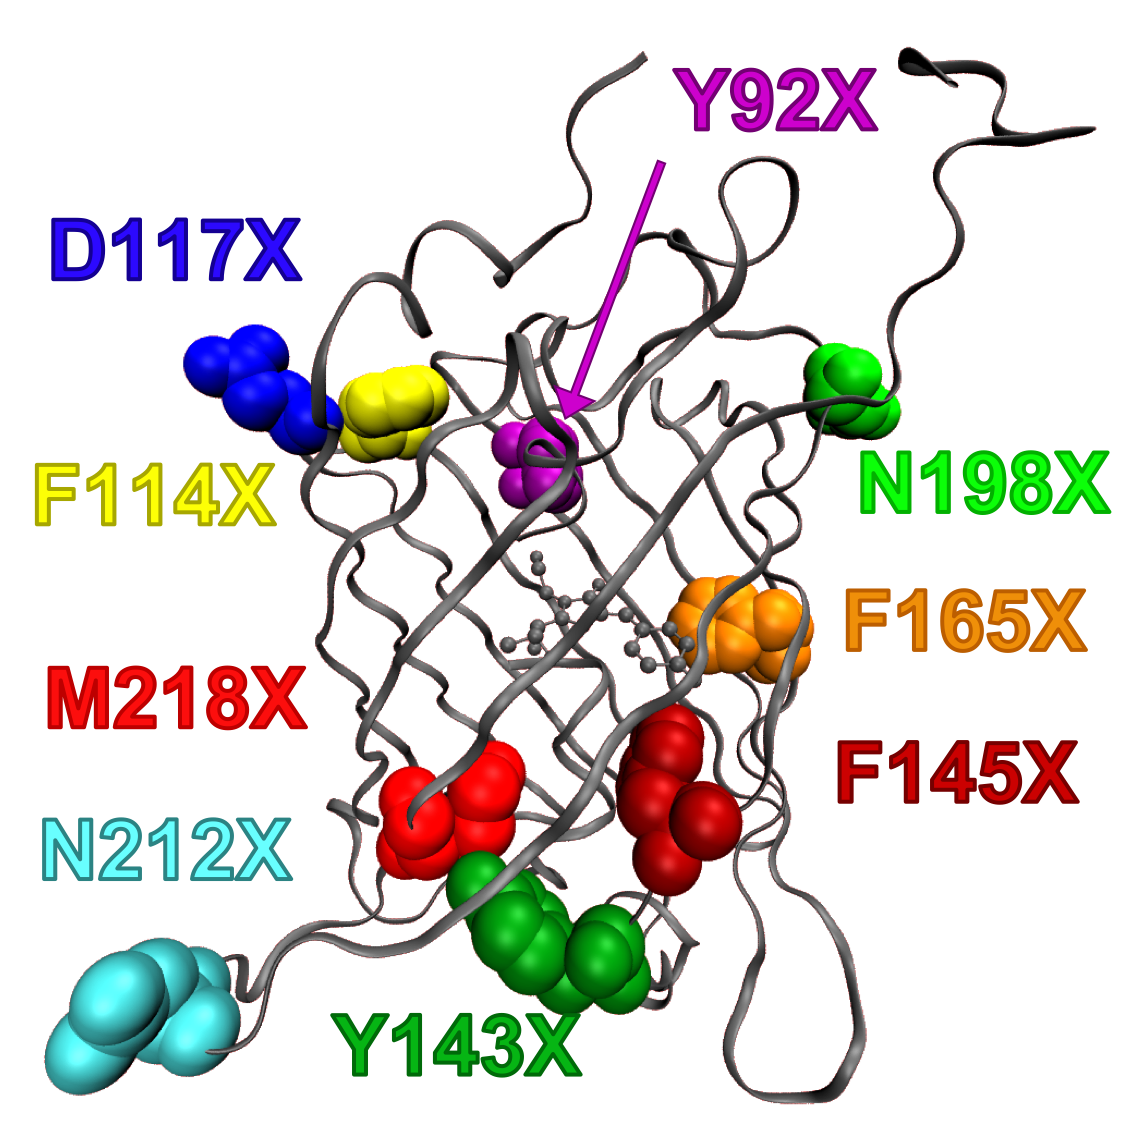
\includegraphics[width=\single]{figures-gfp-hbond/system.png}
    \caption[Locations of the nitrile probes in GFP]{
        Locations of the nitrile probes in green fluorescent protein (GFP) shown on the crystal structure 2b3p. 
        Each location shown in the spherical representations was independently mutated to \emph{p}-cyanophenylalanine (CNF). 
        The first letter indicates the one-letter amino acid code of the residue that was replaced by CNF, denoted by ``X''.
    }
    \label{fig:hbond-system}
\end{figure}

%%%%%%%%%%%%%%%%%%%%%%%%%%%%%%%%%%%%%%%%%%%%%%%%%%%%%%%%%%%%%%%%
%%%%%%%%%%%%%%%%%%%%%%%%%%%%%%%%%%%%%%%%%%%%%%%%%%%%%%%%%%%%%%%%
\section{Methods}\index{hbond-methods}
%%%%%%%%%%%%%%%%%%%%%%%%%%%%%%%%%%%%%%%%%%%%%%%%%%%%%%%%%%%%%%%%
%%%%%%%%%%%%%%%%%%%%%%%%%%%%%%%%%%%%%%%%%%%%%%%%%%%%%%%%%%%%%%%%

%\subsection{Protein Expression and Purification}
%
%A pBAD vector containing the gene for 6xHis-tagged superfolder GFP (Addgene plasmid \#85482) and a pDule vector containing a tRNA synthetase/tRNA pair evolved for CNF (Addgene plasmid \#85494) were kindly provided by the Mehl group \cite{Miyake-Stoner2009, Miyake-Stoner2010}.
%Amber codons were introduced into the superfolder GFP (hereafter, simply GFP) gene at the desired locations, and the amber-coded pBAD vector was co-transformed alongside the pDule vector into DH10\textbeta{} cells.
%Single colonies from plates containing ampicillin and tetracycline were used to seed the growth of 1 L cultures in an autoinduction media described by Mehl et al \cite{Hammill2007}.
%After 24-30 h of expression, cells were harvested and either purified immediately or stored at -80 \si{\celsius} until further use.
%6xHis-tagged GFP mutants containing CNF were purified by immobilized metal affinity chromatography, and the 6xHis tags were cleaved with trypsin proteolysis.
%Cleaved GFP mutants were buffer exchanged into degassed phosphate buffered saline (PBS) at pH 7.4 and used immediately or stored at -80 \si{\celsius}. 
%
%\subsection{FTIR Spectroscopy}
%
%Nitrile-containing GFP mutants were concentrated to $\sim$2 mM using Amicon Ultra 10 000 molecular weight cutoff filters according to the manufacturer's protocol.
%Following concentration, samples were spun for 5 minutes at 15 000 rpm to remove any air bubbles.
%Samples were injected into a temperature-controlled cell at 5 \si{\celsius} between two sapphire windows separated by two 100 $\mu$m teflon spacers.
%Spectra were recorded at 5, 15, 25, and 35 \si{\celsius}, in that order, averaging over 600 scans at a resolution of 0.5 \si{\wn}, allowing the sample to equilibrate for at least 10 minutes before scanning at each temperature.
%At the end of the 35 \si{\celsius} measurement, the intact cell was cleaned with water and ethanol, and then PBS was added to the 35 \si{\celsius} equilibrated cell for background spectra, which were collected in the reverse order of temperature to avoid the formation of air bubbles during the scans.

\subsection{Molecular Dynamics Simulations}

A template protein was modeled by homology from the 2b3p crystal structure\cite{Pedelacq2006} using a procedure described elsewhere \cite{Slocum2017}.
Using this template, nine separate mutations from the WT residue to phenylalanine were made using the mutagenesis wizard tool in PyMol\cite{DeLano2002} at each of the CNF locations.
Using the Avogadro molecular editing package \cite{Hanwell2012}, the mutated phenylalanine residue was further modified to CNF and independently minimized.
Parameters for the internal GFP fluorophore were kindly provided by Riccardo Nifos\'i \cite{Nifosi2003}, and parameters for the CNF chromophore have been described previously \cite{Slocum2017}.
All further minimizations and MD simulations were performed using the Gromacs 5.0.4 molecular dynamics simulation package \cite{VanDerSpoel2005, Abraham2015}, and the Amber03 force field (ffAmber03) \cite{Duan2003, Sorin2005}. 

Each of the nine protein systems was energy minimized in vacuum using the steepest descent algorithm and then solvated in a dodecahedron box of TIP3P water \cite{Jorgensen1983}, with a minimum distance of protein to the edge of the box of 1.5 nm.
The solvated systems were then energy minimized using a steepest descent approach, and then heated under the NVT ensemble at 300 K, and equilibrated under the NPT ensemble at 1 atm.
Production MD was run on each equilibrated protein system for 50 ns, using the same simulation parameters as described previously \cite{Slocum2017}, and a snapshot was saved every 4 ps.
The first 10 ns was discarded as equilibration time, and only the last 40 ns was used in the analyses that follow.

%%%%%%%%%%%%%%%%%%%%%%%%%%%%%%%%%%%%%%%%%%%%%%%%%%%%%%%%%%%%%%%%
%%%%%%%%%%%%%%%%%%%%%%%%%%%%%%%%%%%%%%%%%%%%%%%%%%%%%%%%%%%%%%%%
\section{Results}\index{hbond-results}
%%%%%%%%%%%%%%%%%%%%%%%%%%%%%%%%%%%%%%%%%%%%%%%%%%%%%%%%%%%%%%%%
%%%%%%%%%%%%%%%%%%%%%%%%%%%%%%%%%%%%%%%%%%%%%%%%%%%%%%%%%%%%%%%%
\subsection{Vibrational Absorption Measurements}

We measured the nitrile stretching frequencies of biosynthetically incorporated CNF probes at nine positions in GFP, as well as CNF in water and \emph{p}-tolunitrile in THF.
The resulting spectra at 25 \si{\celsius} are shown in Figure \ref{fig:hbond-spectra}, where the number to the right of each spectrum indicates the position of the probe according to Figure \ref{fig:hbond-system}.
Each spectrum was fit to a gaussian curve using an in-house fitting program described elsewhere \cite{Ragain2012}.
The mean vibrational frequency and fwhm of each spectrum are found in Table \ref{tbl:hbond-IR_summary}.
Most of the probe locations (114, 117, 143, 198 and 212) had mean vibrational frequencies that were centered around the value of CNF in water ($\sim$2238 \si{\wn}).
These five probe locations also had similar peak widths (measured as fwhm) to that of CNF in water ($\sim$10 \si{\wn}).
Two probe locations (165 and 218) had mean vibrational frequencies that were shifted to lower frequencies ($\sim$2234 \si{\wn} and $\sim$2231 \si{\wn}, respectively), but were still blue-shifted relative to \emph{p}-tolunitrile in THF.
These two locations had narrower peak widths ($\sim$8 \si{\wn} and $\sim$7 \si{\wn}, respectively).
One probe location (145) had a mean vibrational frequency of $\sim$2225 \si{\wn} and had the narrowest peak width ($\sim$5 \si{\wn}), which is both lower in frequency and narrower than \emph{p}-tolunitrile in THF.
The final probe location (92) had a mean vibrational frequency higher (2243 \si{\wn}) than that of CNF in water and the largest peak width of 12 \si{\wn}.
The range of measured frequencies of the nitrile in these locations is larger than the range for the small CNF analogs in THF (2228 \si{\wn}) and water (2238 \si{\wn}), which are the two solvents commonly used to represent the extremes of potential solvent hydrogen bonding for CNF.
Clearly, the broad range of hydrogen bonding environments available within a complex protein system is not adequately recapitulated by the solvatochromism of small nitrile derivatives. 

\begin{figure}
    \center
    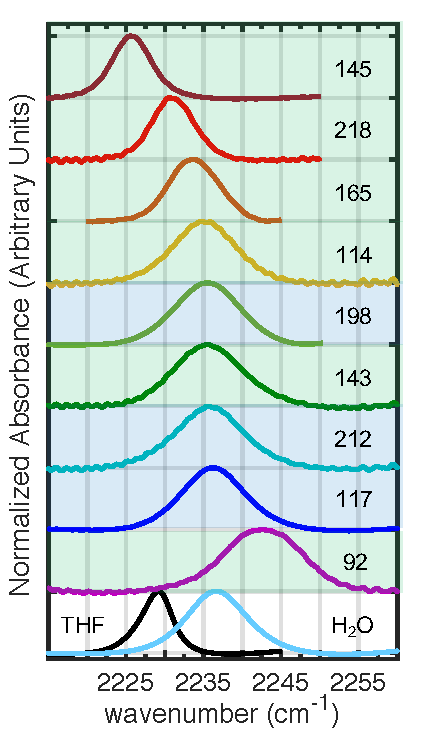
\includegraphics[width=\single]{figures-gfp-hbond/spectra_colors.pdf}
    \caption[FTIR spectra of CNF at each nitrile location]{
        Representative FTIR absorption spectra of CNF in each of the nine locations at 25 \si{\celsius}, arranged from the lowest to highest mean frequency. 
        Each spectrum is normalized to a maximum absorbance of 1. 
        The nitrile location for each spectrum is indicated by the number to the right, according to Figure \ref{fig:hbond-system}. 
        The spectra are offset from the $x$-axis for clarity. 
        The color of the background indicates our \emph{a priori} classification of the solvent accessibility of the nitrile location based on the crystal structure. 
        Blue indicates a position where the wild type side chain is pointed away from the interior of the barrel, and thus the nitrile was expected to be solvent exposed. 
        Green indicates a position where the wild type side chain is pointed into the interior of the barrel, and thus the nitrile was expected to be buried. 
        At the bottom are representative spectra of \emph{p}-tolunitrile in THF at 25 \si{\celsius} (black) and CNF in water at 25 \si{\celsius} (light blue).
    }
    \label{fig:hbond-spectra}
\end{figure}

\begin{table}
    \caption[Summary of experimental spectra]{A summary of the mean vibrational frequencies and FWHM of the nine different nitrile locations at each of the four temperatures.}
    \begin{center}
        %\begin{adjustbox}{angle=90}
        \begin{tabular}{c|cc|cc}
            \toprule
            \multirow{2}{*}[-2pt]{CNF location} &   \multicolumn{2}{c}{5 \si{\celsius}}   &         \multicolumn{2}{c}{15 \si{\celsius}} \\
            \cmidrule[0.2pt](){2-5}
            
                 & Mean Freq.  & FWHM & Mean Freq. & FWHM\\ 
            \midrule
            92   & 2243.7  & 11.4 & 2243.2 & 11.7 \\
            114  & 2235.6  & 10.2 & 2235.4 & 10.1 \\
            117  & 2237.0  & 11.5 & 2236.6 & 10.4 \\
            143  & 2236.2  & 10.8 & 2235.9 & 10.7 \\
            145  & 2226.1  & 6.2  & 2225.9 & 6.3  \\
            165  & 2234.1  & 7.9  & 2233.9 & 7.8  \\
            198  & 2235.9  & 10.1 & 2235.7 & 10.2 \\
            212  & 2236.7  & 10.9 & 2236.3 & 10.7 \\
            218  & 2231.7  & 6.8  & 2231.4 & 6.7  \\

            \midrule   
            \multirow{2}{*}[-2pt]{CNF location} &   \multicolumn{2}{c}{25 \si{\celsius}}       &    \multicolumn{2}{c}{35 \si{\celsius}}    \\
            \cmidrule[0.2pt](){2-5}
             & Mean Freq. & FWHM &  Mean Freq. & FWHM \\
             \midrule

            92   & 2242.6 & 12.2 &  2241.9 & 12.2 \\
            114  & 2235.1 & 10.0 &  2234.8 & 10.4 \\
            117  & 2236.3 & 9.8  &  2235.9 & 9.5  \\
            143  & 2235.6 & 10.9 &  2235.2 & 11.0 \\
            145  & 2225.7 & 6.4  &  2225.5 & 6.6  \\
            165  & 2233.7 & 7.7  &  2233.6 & 7.5  \\
            198  & 2235.5 & 10.0 &  2235.2 & 9.7  \\
            212  & 2235.7 & 10.7 &  2235.1 & 11.1 \\
            218  & 2231.0 & 6.7  &  2230.7 & 6.6  \\




            \bottomrule
            
            \end{tabular}
        %\end{adjustbox}
    \end{center}
    \label{tbl:hbond-IR_summary}
\end{table}

Next, we measured the temperature dependence of the nitrile stretching frequencies for each of the nine positions in GFP, as well as CNF in water and \emph{p}-tolunitrile in THF, over the range of 5-35 \si{\celsius}.
Over this temperature range, GFP has been shown be to remain stably folded \cite{Slocum2016, Pedelacq2006}.
The mean vibrational frequency and fwhm of each spectrum at each temperature are also found in Table \ref{tbl:hbond-IR_summary}.
Figure \ref{fig:hbond-ftls} shows the change in nitrile center frequency (relative to the frequency at 5 \si{\celsius}) as a function of temperature.
Similar to the work of Adhikary et al. \cite{Adhikary2015}, we measured a linear response over this temperature range for each of the probe locations, as well as for the small molecules.
For the aprotic solvent THF, we did not measure any change in the nitrile stretching frequency over this temperature range (Figure \ref{fig:hbond-ftls}, black).
Conversely, for CNF in water we measured a large change in frequency as a function of temperature (Figure \ref{fig:hbond-ftls}, light blue).
Interestingly, each nitrile location in our nine systems had a distinct FTLS, showing that our nine protein systems sampled a broad range of different hydrogen bonding interactions.
Most of the CNF probes in GFP gave temperature responses that were in between the extremes of THF and water, which suggests that these probes all experience varying amounts of hydrogen bonding that are not as strong as the well-solvated CNF in water.
However, for the nitriles at positions 212 and 92, we measured a FTLS greater than that for CNF in water, possibly suggesting that these two probe locations experience either more frequent, or stronger, hydrogen bonds than CNF in water.
This is not surprising for position 212, which is on a solvent exposed loop in GFP (Figure \ref{fig:hbond-system}).
However, position 92 is pointed into the GFP barrel, where we do not expect much interaction between the nitrile and water.
To interpret the differences in the FTLS of the nitrile in different locations, we turned to MD simulations to investigate the local hydrogen bonding interactions around each probe, including to the nitrile itself. 

\begin{figure}
    \center
    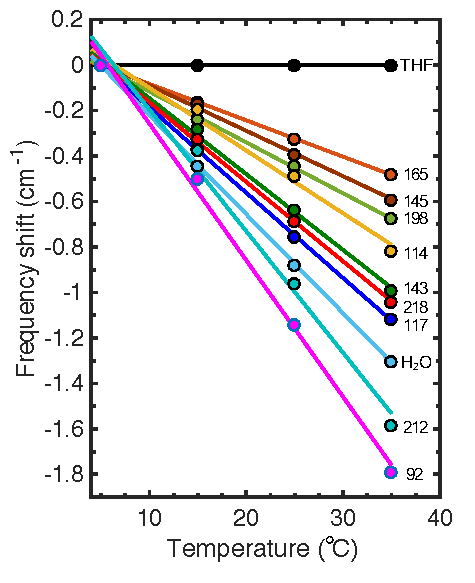
\includegraphics[width=\single]{figures-gfp-hbond/FTLS.pdf}
    \caption[FTLS measurements of each nitrile]{
        Mean vibrational frequencies of CNF at each location as a function of temperature. 
        The number to the right indicates the CNF location according to Figure \ref{fig:hbond-system}. 
        Linear regression was used to fit a line to each data set. 
        The slope of each trend line is the FTLS for that particular probe location. 
        The temperature dependencies of the mean vibrational frequency of CNF in water (light blue) and \emph{p}-tolunitrile in THF (black) are also shown.
    }
    \label{fig:hbond-ftls}
\end{figure}

\subsection{SASA calculations}

In principle, the hydrogen bonding environment of a probe at any location could be investigated in a straightforward way through atomistic simulations.
One easy and popular choice for quantifying solvent exposure to specific residues within a protein is with the SASA of the amino acid.
However, SASA calculations suffer from the major disadvantage that they lack molecular details about solvent interactions.
Specifically, they do not include information about geometric orientations of hydrogen bonding, and they do not capture interactions that arise when a residue is not exposed to bulk solvent, such as those from confined waters or from the protein itself.
Nevertheless, SASA serves as a good first approximation to a measurement of hydrogen bonding interactions to the nitrile probe.  
Using the gmx sasa tool \cite{Eisenhaber1995}, we calculated the SASA of several subsets of the atoms within the CNF residue over the course of the 40 ns of production MD simulation for each GFP mutant. 
Specifically, we calculated the SASA of the nitrile alone, the nitrile plus the C$_{\beta}$, two H$_{\beta}$s and the phenyl ring, and the entire CNF residue including the backbone atoms.
The subsets for these calculations are illustrated in Figure \ref{fig:hbond-sasa_regions}, and the results are shown in Figure \ref{fig:hbond-sasa_regions_v_time}.
We found that the SASA of just the nitrile with its low total surface area was very sensitive to small changes in the surrounding protein structure, giving large fluctuations in SASA over the course of the simulation.
The SASA of the entire residue, shown in Figure \ref{fig:hbond-sasa}, gave the broadest range of values with the smallest standard deviations.
We have therefore chosen to focus on these values for the analysis that follows.
Across each of the nine CNF locations, there was a continuum of SASA possibilities ranging from completely solvent exposed to completely inaccessible.
SASA calculations revealed that two probes (positions 117 and 212) were highly solvent exposed and had SASAs that approached the calculated maximum of CNF by itself in solvent ($\sim$2.5 nm$^2$).
Three probes, at positions 114, 143 and 198, had intermediate SASAs ($\sim$0.5 nm$^2$ to 1.5 nm$^2$) relative to free CNF.
Two probes (positions 145 and 165) had a low SASA ($\sim$0.25 nm$^2$ to 0.5 nm$^2$) relative to free CNF.
Finally, two probes (positions 92 and 218) showed nearly zero SASA throughout the simulation, though these two had quite different FTLS values, shown in Figure \ref{fig:hbond-ftls}.
This discrepancy between the SASA and the measured FTLS suggests that the nitriles in these nine positions experienced differences in local environment more complex than could be captured by SASA calculations.

\begin{figure}
    \center
    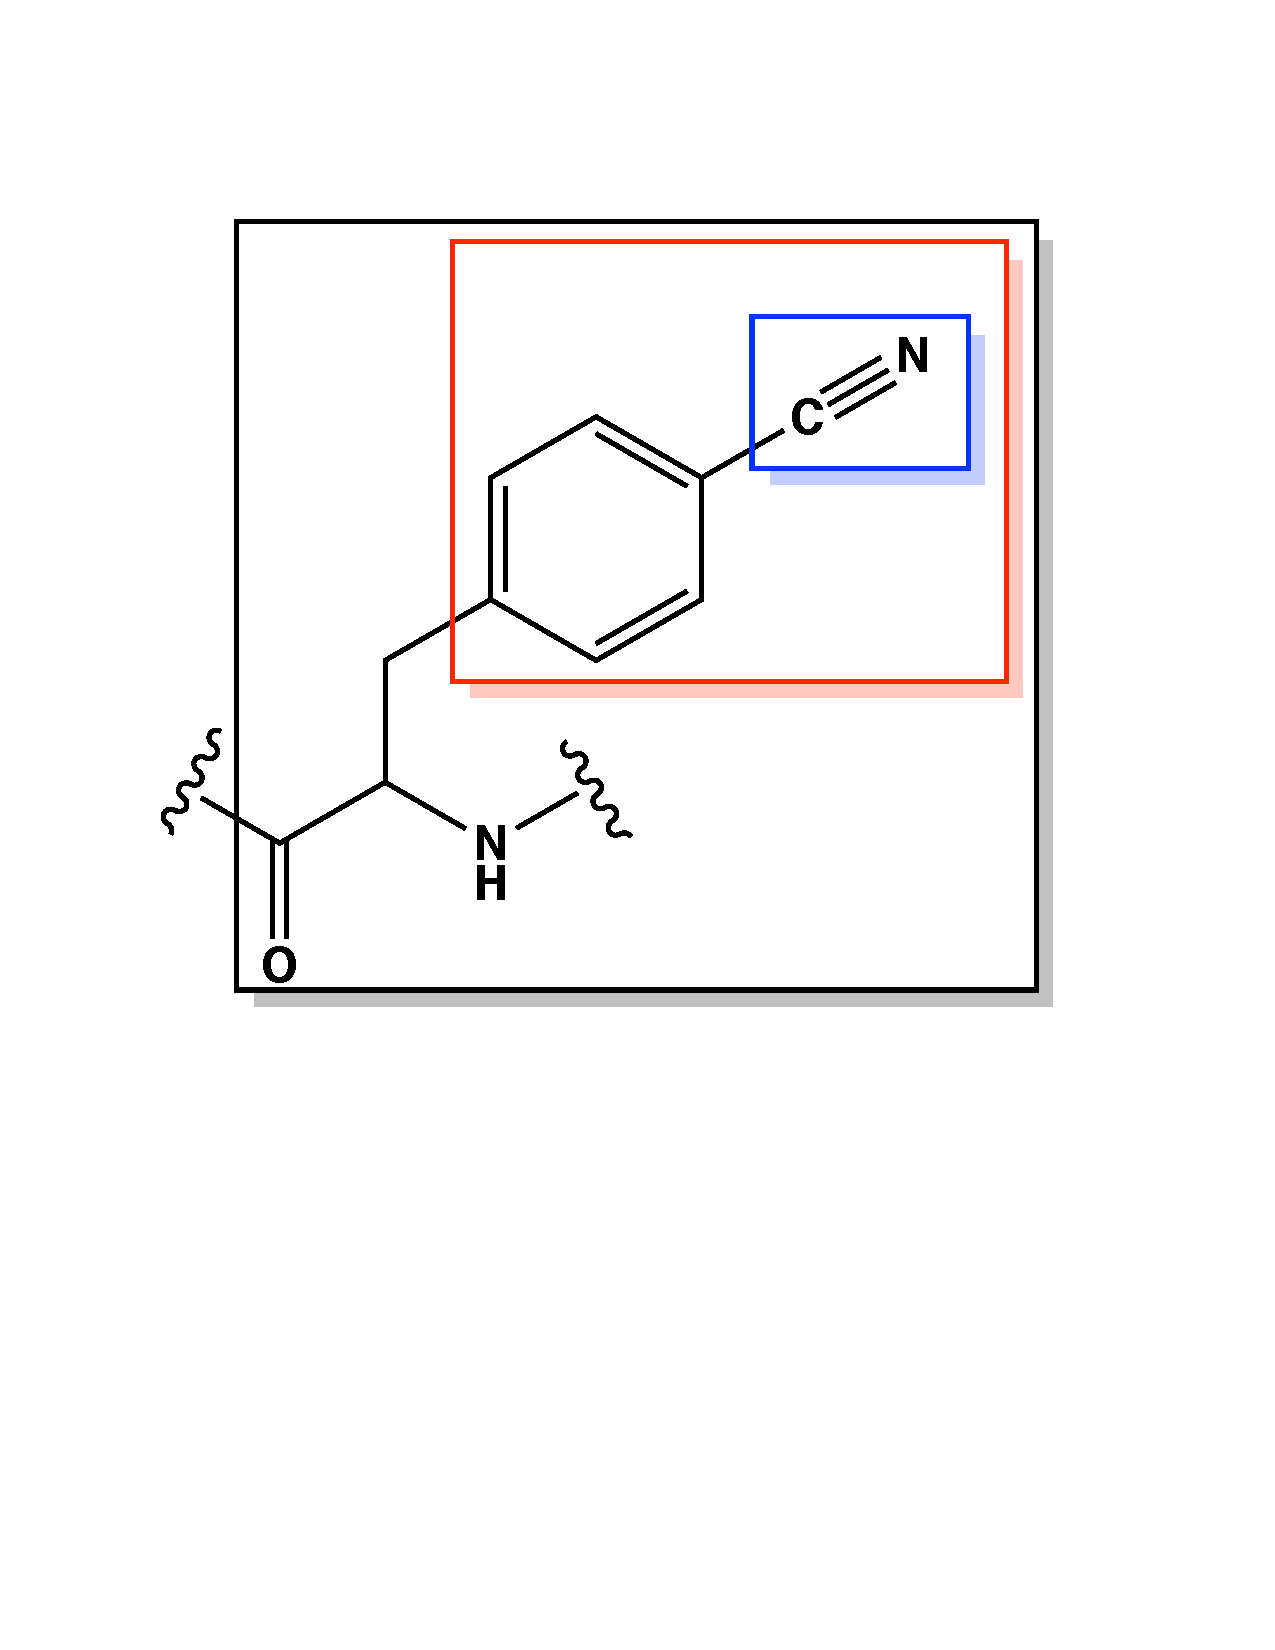
\includegraphics[width=\single]{figures-gfp-hbond/sasa_regions_aromatic.pdf}
    \caption[Schematic of regions used for SASA calculations]{
        SASA calculations and analyses were carried out for each of the three highlighted regions. 
        In blue, the SASA of only the nitrile group was calculated. 
        In red, the SASA of the nitrile group and the atoms of aromatic ring was calculated. 
        In black, all atoms (including those of the amide backbone) were included in the SASA calculation. 
        The set of atoms highlighted in black are the atoms used for the calculations discussed and presented in the text.
    }
    \label{fig:hbond-sasa_regions}
\end{figure}

\begin{figure}
    \center
    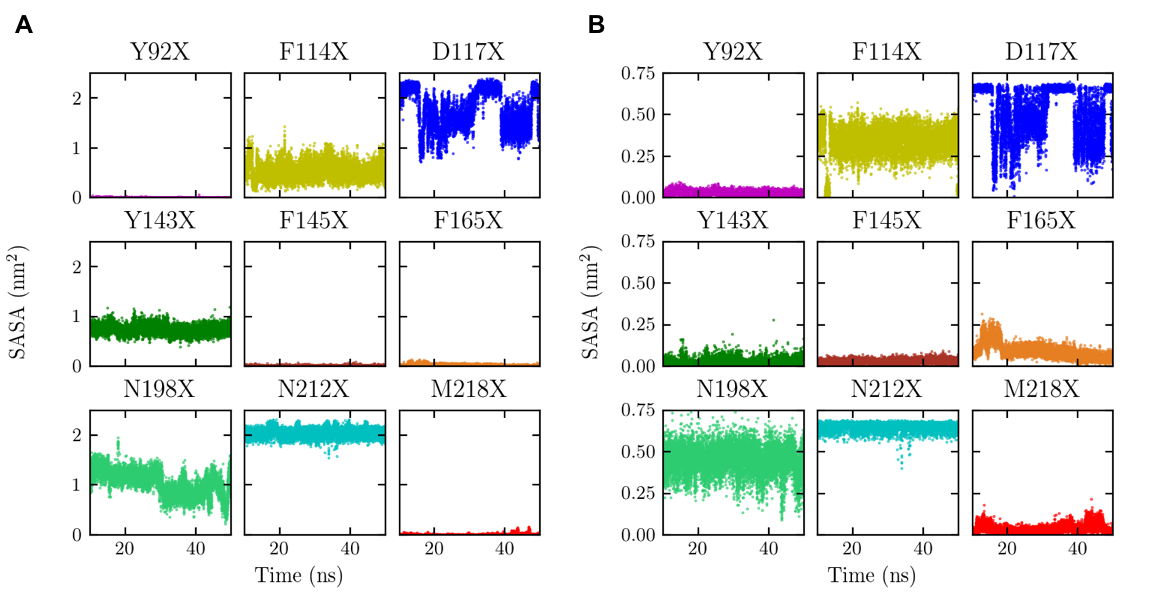
\includegraphics[width=\double]{figures-gfp-hbond/FigureS1_combined.png}
    \caption[Calculated SASA of smaller subsets of atoms of CNF]{
        The SASA of the two different subsets of atoms of the CNF residue as a function of simulation time in 40 ns of production MD simulation for the nine GFP mutants containing the nitrile group. 
        (A) The SASA was calculated over the aromatic ring and the nitrile group. 
        This subset of atoms is highlighted by the red box in Figure \ref{fig:hbond-sasa_regions}. 
        (B) The SASA was calculated over only the atoms in the nitrile group. 
        This subset of atoms is highlighted by the blue box in Figure \ref{fig:hbond-sasa_regions}.
    }
    \label{fig:hbond-sasa_regions_v_time}
\end{figure}

\begin{figure}
    \center
    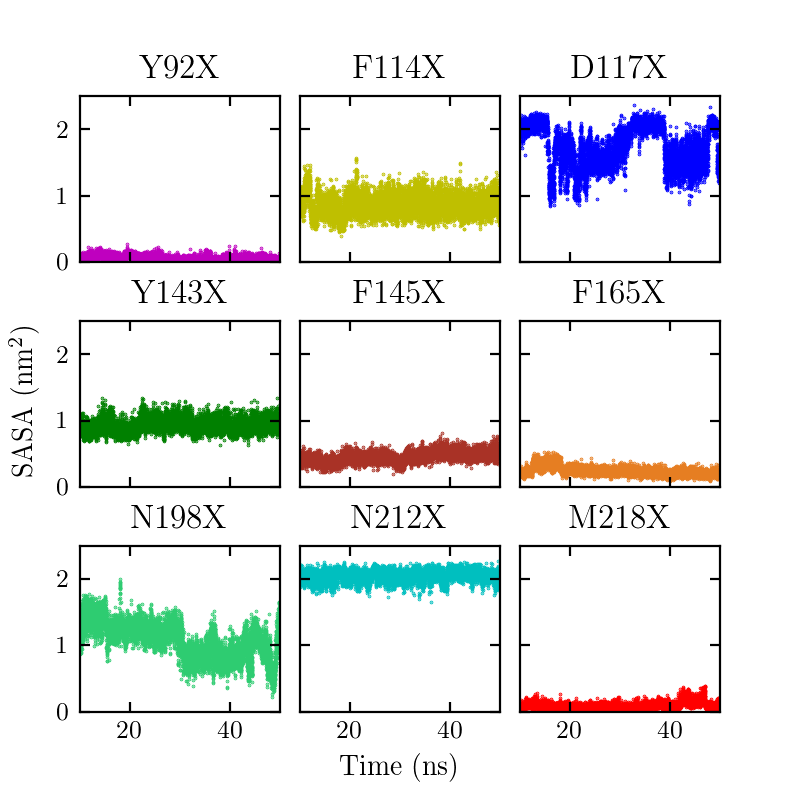
\includegraphics[width=\single]{figures-gfp-hbond/sasa_v_time.png}
    \caption[Calculated SASA of entire CNF residue over the course of the MD simulation]{
        SASA of the CNF residue as a function of simulation time in 40 ns of production MD simulation for the nine GFP mutants containing the nitrile group.
    }
    \label{fig:hbond-sasa}
\end{figure}

\subsection{Hydrogen bonding calculations}

The MD simulations provide molecular level information about the hydrogen bonds around each nitrile probe that is significantly more detailed than the SASA.
For each of the nine systems, we analyzed the MD trajectories for the presence and geometry of hydrogen bonding using an in-house code to characterize hydrogen bonds to a nitrile probe in each frame of the simulation.
All nearby O, N, S, and C$_{\alpha}$ atoms were considered to be potential donors.
A hydrogen bond donor was determined to be hydrogen bonding if three conditions were satisfied: 1) the C--N$\cdots$H angle was greater than \ang{99} ($\theta_1$ in Figure \ref{fig:hbond-scheme}); 2) the N$\cdots$H--R$_{\text{donor}}$ angle ($\theta_2$ in Figure \ref{fig:hbond-scheme}) was greater than \ang{120}; and 3) the N$\cdots$H distance was less than 2.45 \si{\angstrom} ($d_{\text{NH}}$ in Figure \ref{fig:hbond-scheme}).
These cutoff values were chosen to accept hydrogen bonds that fall within 2 standard deviations of a typical hydrogen bond to nitriles, as defined by Le Questel et al \cite{LeQuestel2000}.
The code was implemented in C++ for use with the Gromacs package.  

\begin{figure}
    \center
    
\includegraphics[width=\single]{figures-gfp-hbond/hbonding_scheme.png}
    \caption[Schematic of the hydrogen bonding geometric criteria]{
        Schematic of the hydrogen bonding geometric criteria. 
        $\theta_1$ is the C--N$\cdots$H angle. 
        $\theta_2$ is the N$\cdots$H--R$_{\text{donor}}$ angle, where R$_{\text{donor}}$ represents any hydrogen bond donor. 
        $d_{\text{NH}}$ is the distance between the hydrogen and the acceptor nitrogen. 
        In this analysis, any O, N, S, C$_{\alpha}$ atom was considered to be a potential hydrogen bond donor. 
        To be considered a hydrogen bond, $\theta_1$ must be greater than \ang{99}, $\theta_2$ must be greater than \ang{120}, and $d_{\text{NH}}$ must be less than 2.45 \si{\angstrom}.
    }
    \label{fig:hbond-scheme}
\end{figure}

\subsection{Hydrogen bonds donated from water}

Hydrogen bonding interactions between the nitrile and water were analyzed for each snapshot of the nine MD simulations of CNF containing variants.
For each hydrogen bond, the geometry was calculated, and the different geometries were binned by $\theta_1$ and $d_{\text{NH}}$.
These results are plotted as heat maps in Figure \ref{fig:hbond-heatmap}A.
Hydrogen bonding geometries were also binned according to $\theta_2$ and $d_{\text{NH}}$.
However, the $\theta_2$ and $d_{\text{NH}}$ distributions (Figure \ref{fig:hbond-heatmap}) did not vary greatly across the nine systems (data not shown), and therefore contained less information.
For the rest of these analyses, we will focus primarily on $\theta_1$ as the determinant angle.
Figure \ref{fig:hbond-heatmap}A shows that several different hydrogen bonding geometries between the nitrile probes and water were present in our MD simulations.
The nitriles at positions 114, 117, 198, and 212 experienced broad distributions of hydrogen bonding angles, with each distribution covering the entire range of allowed angles (\ang{99} to \ang{180}).
This type of hydrogen bonding profile is consistent with a large degree of solvent exposure, where the hydrogen bonds are free to take on many orientations.
A representative snapshot of CNF in a solvent exposed position is shown in Figure \ref{fig:hbond-snapshot}A.
In contrast, Figure \ref{fig:hbond-heatmap}A shows the nitriles at position 145 and 218 experienced a much narrower distribution of hydrogen bonds, with hydrogen bonding angles localized between \ang{110} and \ang{150}.
A representative snapshot of a hydrogen bond between water and CNF 145 is shown in Figure \ref{fig:hbond-snapshot}B, and a representative snapshot of a hydrogen bond between water and CNF 218 is shown in Figure \ref{fig:hbond-snapshot}C.
These specific hydrogen bond geometries will be discussed in more detail below.
The nitriles at positions 92 and 143 experienced very few hydrogen bonds from water throughout the simulation (Figure \ref{fig:hbond-heatmap}A).
The nitrile at position 165 experienced slightly more hydrogen bonding from water than position 92 and 143, with two distinct geometries, one centered near \ang{150} and one centered near \ang{100} (Figure \ref{fig:hbond-heatmap}A).
Even using only three geometric parameters and considering only hydrogen bonds from water, we observed that CNF at these nine locations experienced a wide variety of possible hydrogen bonding interactions.
Clearly, a Boolean classification of hydrogen bonding is insufficient to describe the individual positions of each nitrile vibrational probe used in this work. 

\begin{figure}
    \center
    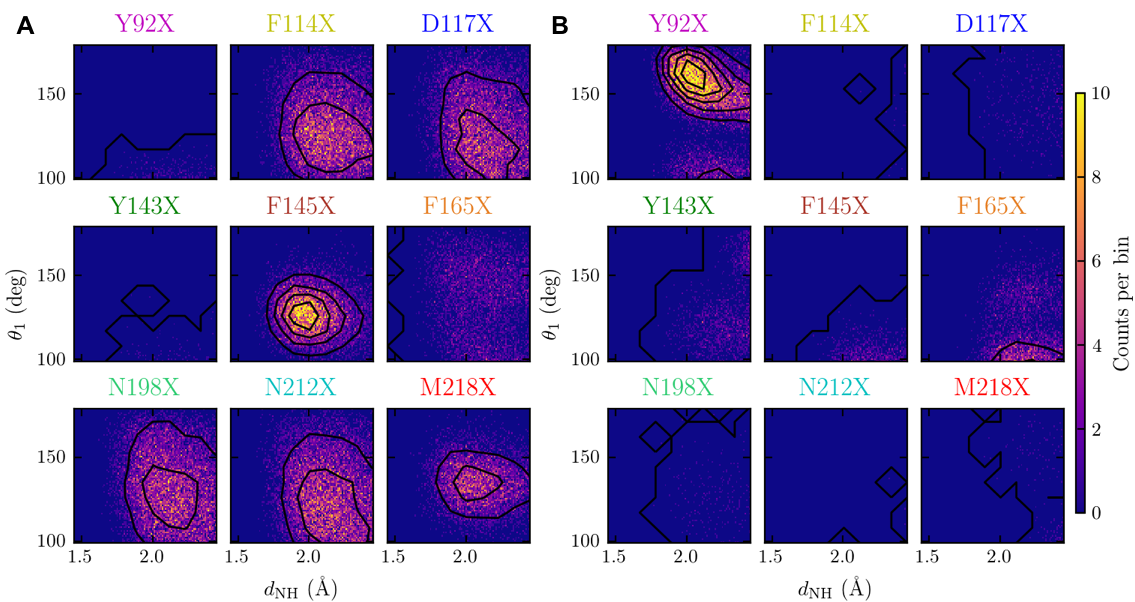
\includegraphics[width=\double]{figures-gfp-hbond/Figure6_combined.png}
    \caption[Heat maps of the hydrogen bonding geometries to CNF at each probe location]{
        Heat maps of the hydrogen bonding geometries to CNF at each probe location. 
        The titles are colored to correspond to the color codes used elsewhere in the paper. 
        The hydrogen bonding geometries to CNF were calculated at each snapshot (every 4 ps) of the last 40 ns of a 50 ns MD simulation. 
        Contour lines are drawn to guide the eye. 
        $d_{\text{NH}}$ ($x$-axis) and $\theta_1$ ($y$-axis) are defined in Figure \ref{fig:hbond-scheme}. 
        (A) Hydrogen bonds that are donated specifically from water, where R$_{\text{donor}}$ is the oxygen atom of a water molecule. 
        (B) Hydrogen bonds that are donated from protein, where R$_{\text{donor}}$ may be any N, O, S, or C$_{\alpha}$ atom on the protein.
    }
    \label{fig:hbond-heatmap}
\end{figure}

\begin{figure}
    \center
    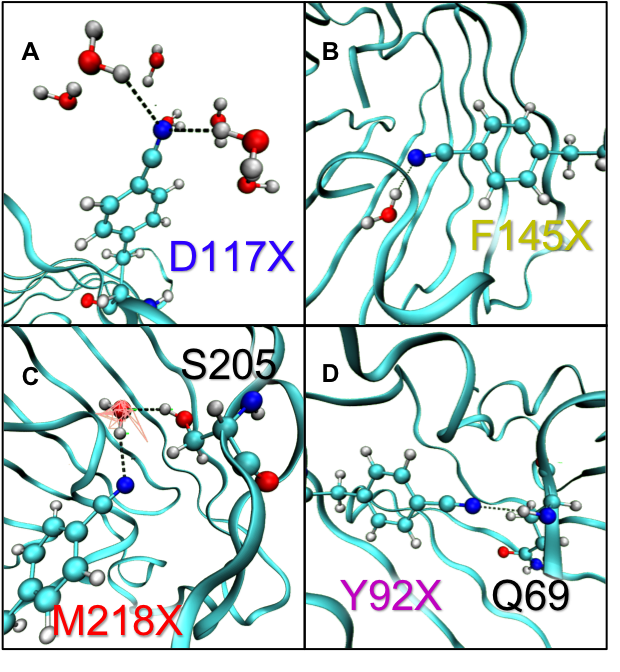
\includegraphics[width=\single]{figures-gfp-hbond/snapshots.png}
    \caption[Representative snapshots of select hydrogen bonding configurations observed in simulation]{
        Representative snapshots of select hydrogen bonding configurations observed in simulation. 
        (A) The nitrile at position 117 was solvent exposed and involved in multiple simultaneous hydrogen bonds that exchanged frequently throughout the simulation. 
        (B) The nitrile at position 145 was involved with a $\pi$-hydrogen bond with a confined water molecule, where $\theta_1$ was approximately \ang{120}. 
        (C) The nitrile at position 218 was involved in a hydrogen bond with a confined water molecule, which is also hydrogen bound to the OH group of Ser205. 
        The Connolly surface computed with gmx sasa is shown in pink lines to emphasize how a small available SASA can still have significant hydrogen bonding. 
        (D) The nitrile at position 92 was involved in a linear hydrogen bond with the amide hydrogen of Gln69, where $\theta_1$ was approximately \ang{180}.
    }
    \label{fig:hbond-snapshot}
\end{figure}

\subsection{Hydrogen bonds donated from protein}

In addition to hydrogen bonds from water, we also investigated possible hydrogen bonds formed between the nitrile and donors from protein moieties.
Specifically, any O, N, S, or C$_{\alpha}$ atom in the protein was considered to be a possible hydrogen bond donor.
For each hydrogen bond between the nitrile and a protein donor, the geometry of the interaction was calculated and binned, and the results are shown as a heat map in Figure \ref{fig:hbond-heatmap}B.
Most nitrile locations (114, 117, 145, 198, 212, and 218) did not experience significant hydrogen bonding to donors from the protein.
However, the nitriles at positions 143 and 165 experienced some hydrogen bonding from the protein, and the nitrile at position 92 experienced extensive hydrogen bonding from a protein donor.
To investigate these protein-donated hydrogen bonding populations, we inspected the trajectories of each nitrile location.
For the nitrile at location 165, we found that the nitrile accepted transient hydrogen bonds from nitrogen atoms on two different nearby side chains (Arg96 and Gln183), leading to the two distinct populations shown in Figure \ref{fig:hbond-heatmap}B.
For the nitrile at position 143, we found that the nitrile accepted hydrogen bonds from a nitrogen on nearby Lys207, and interestingly the nitrile also accepted transient hydrogen bonds from the C$_{\alpha}$ of nearby Met218.
Carbon donated hydrogen bonds, especially from C$_{\alpha}$ atoms to nearby oxygen atoms, are common in proteins and have been under investigation for some time \cite{Wahl1997, Scheiner2011, Horowitz2012}, but this is the first evidence to our knowledge of a carbon-nitrile hydrogen bond.
Finally, at position 92, we found that the nitrile had a high probability of accepting a linear hydrogen bond from the amide hydrogen of Gln69.
A representative snapshot of this interaction is shown in Figure \ref{fig:hbond-snapshot}D and will be discussed in more detail below.
The observation that several of these CNF probes in the interior of GFP were engaged in hydrogen bonds with protein donors leads us to believe that because hydrogen bonds to the nitrile are so energetically favorable, the nitrile will accept weak hydrogen bonds from unconventional donors rather than remain isolated.  

%%%%%%%%%%%%%%%%%%%%%%%%%%%%%%%%%%%%%%%%%%%%%%%%%%%%%%%%%%%%%%%%
%%%%%%%%%%%%%%%%%%%%%%%%%%%%%%%%%%%%%%%%%%%%%%%%%%%%%%%%%%%%%%%%
\section{Discussion}\index{discussion}
%%%%%%%%%%%%%%%%%%%%%%%%%%%%%%%%%%%%%%%%%%%%%%%%%%%%%%%%%%%%%%%%
%%%%%%%%%%%%%%%%%%%%%%%%%%%%%%%%%%%%%%%%%%%%%%%%%%%%%%%%%%%%%%%%

\subsection{Relationship between FTLS and SASA}

To assess if the FTLS is a good measure of hydrogen bonding interactions, we plotted the measured FTLS against the ensemble averaged SASA of the CNF residues from simulation in Figure \ref{fig:hbond-comparison}A.
Our results show that there is a strong correlation between FTLS and SASA ($r = -0.920$), with two outliers (positions 92 and 218) that are not included in the regression fit.
We also performed this analysis using the SASA calculations of the aromatic sidechain atoms and the nitrile alone (from Figure \ref{fig:hbond-sasa_regions_v_time}).
The resulting comparisons can be found in Figure \ref{fig:hbond-regions_v_FTLS}. 
While the trends in Figures \ref{fig:hbond-comparison}A and \ref{fig:hbond-regions_v_FTLS} are consistent, because the relative standard deviations of the SASA increase dramatically as the region of the calculation is reduced, we have chosen to focus on the SASA values calculated for all atoms of the CNF residue.
The correlation between FTLS and SASA indicates that the CNF probes in locations that have higher SASA, and therefore higher potential hydrogen bonding interactions with water, show a greater change in the nitrile absorption frequency as temperature is changed.
The two outliers of positions 92 and 218 experienced hydrogen bonds that are not well described by SASA calculations and will be discussed in more detail below.
The SASA calculations for position 117 and 198 have larger standard deviations than the rest of the data.
Examining snapshots from the MD simulations revealed that CNF 117 alternated between two states with different SASAs through a torsional rotation about $\chi_1$ of CNF.
Similarly, CNF 198 drifted from a state of high SASA to a state of lower SASA over the course of the simulation.
These two examples of complex dynamic behavior of the CNF side chain indicate that enhanced MD sampling of CNF and/or its environment could lead to an even more quantitative relationship between SASA and FTLS; we are currently investigating this hypothesis. 

\begin{figure}
    \center
    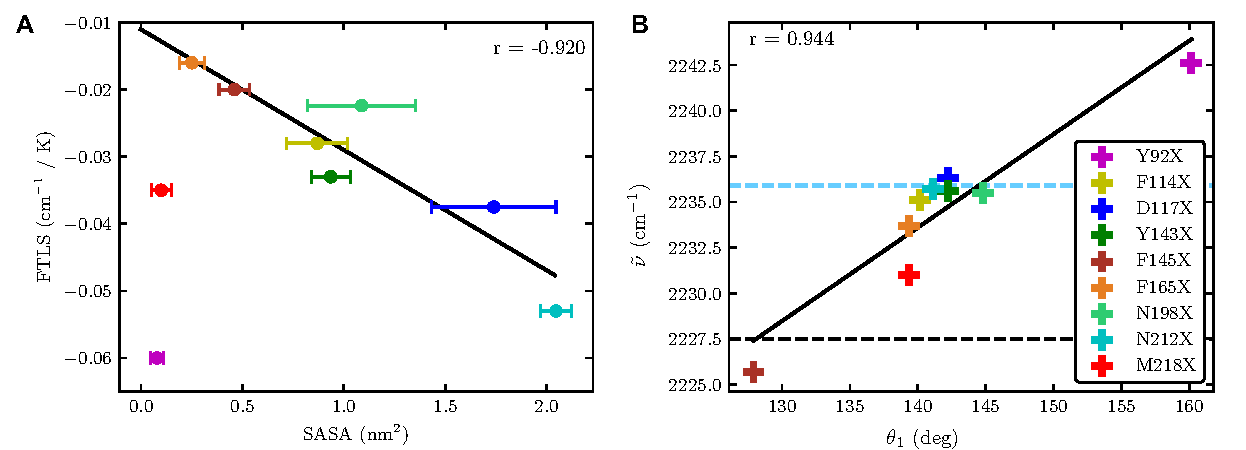
\includegraphics[width=\double]{figures-gfp-hbond/Figure8_combined.pdf}
    \caption[Comparison of calculated properties (SASA and hydrogen bonding angle) against experimental counterparts (FTLS and nitrile frequency)]{
        (A) The ensemble averaged SASA of the CNF residue plotted against the measured FTLS. 
        The error bars on the $x$-axis are the standard deviations of the calculated SASAs. 
        The regression line (black) does not include the nitrile at position 92 (purple) or 218 (red). 
        These outliers are discussed in the main text. 
        (B) For each of the nine nitrile locations, the average angle of hydrogen bonding from simulation is plotted against the experimental mean vibrational frequency. 
        For reference, the mean vibrational frequency of CNF in water is shown as a light-blue dashed line, and the mean vibrational frequency of \emph{p}-tolunitrile in THF is shown as a black dashed line. 
        All vibrational frequencies shown here were measured at 25\si{\celsius}.
    }
    \label{fig:hbond-comparison}
\end{figure}

\begin{figure}
    \center
    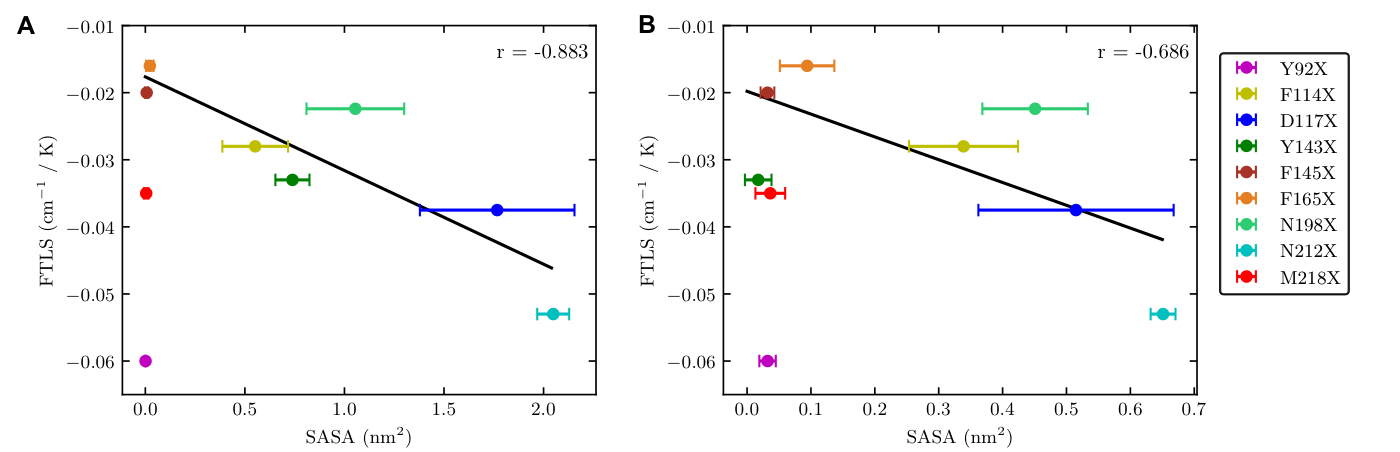
\includegraphics[width=\double]{figures-gfp-hbond/FigureS3_combined.png}
    \caption[Calculated SASA of smaller subsets of atoms against the measured FTLS]{
        The ensemble averaged SASA of the CNF residue plotted against the measured FTLS. 
        The error bars on the $x$-axis are the standard deviations of the calculated SASAs. 
        The regression line (black) does not include the nitrile at position 92 (purple) or at 218 (red). 
        These outliers are discussed in the text. 
        (A) The calculated SASA is taken over the aromatic ring and the nitrile group (highlighted in red in Figure \ref{fig:hbond-sasa_regions}). 
        (B) The calculated SASA is taken over only the nitrile group (highlighted in blue in Figure \ref{fig:hbond-sasa_regions}).
    }
    \label{fig:hbond-regions_v_FTLS}
\end{figure}

It is important to note that not all hydrogen bonding environments are captured by a calculation of the SASA.
For the two outliers discussed previously, CNF 92 and 218, we saw that the nitriles in these two locations experienced hydrogen bonding interactions that were not well described by SASA.
The data in Figure \ref{fig:hbond-heatmap} clearly demonstrate that CNF 92 was involved in a strong linear hydrogen bond with the amide hydrogen of Gln69, a representative snapshot of which is shown in Figure \ref{fig:hbond-snapshot}D.
Since this interaction was not due to solvent, it was not captured by the SASA.
In this case, relying only on the SASA calculation would have resulted in the incorrect conclusion that this nitrile was in an environment free from hydrogen bonding.
The FTLS, however, was the largest of any of the probe locations.
This leads us to believe that nitriles in buried locations as predicted by the calculation of SASA can still be involved in significant hydrogen bonding, and that SASA should not solely be relied upon for evaluating the hydrogen bonding potential of a probe location.
Further, we believe that this shows that in such cases the FTLS still provides a good experimental measure of hydrogen bonding interactions of the nitrile.
Because the FTLS was large over the temperature range measured in this particular case, we hypothesize that at increased temperatures, the thermal fluctuations of the protein backbone will increase and break the linear hydrogen bond between CNF 92 and the protein backbone, resulting in a large FTLS. 

Additionally, CNF 218 had a very low SASA, but the data in Figure \ref{fig:hbond-heatmap}A clearly show extensive hydrogen bonding to the solvent.
While the entire residue was surrounded by protein, leading to low SASA values, the nitrile group itself pointed directly to a single confined water stabilized by a hydrogen bond to Ser205, a representative snapshot of which is shown in Figure \ref{fig:hbond-snapshot}C.
This water formed hydrogen bonds with CNF 218 and could not easily diffuse away from the nitrile when the hydrogen bond was broken.
While the water molecule exchanged throughout the simulation, it did so rarely.
Because the small SASA was occupied with a hydrogen bonding water molecule, the calculated SASA underestimated the hydrogen bonding interactions.
In this case again, relying solely upon the calculated SASA would have led to the incorrect conclusion that this nitrile location was free from hydrogen bonding, while the measured FTLS still captured the hydrogen bonding interactions.
We interpret the FTLS of CNF 218 to indicate that this water is more likely to exchange with increased temperature, weakening the hydrogen bonding interaction to the nitrile and shifting the frequency.
We are currently investigating both of these hypothesized interpretations of the FTLS with additional simulations at varying temperatures.

These two observations from the MD trajectories of CNF 92 and 218 provide clear and direct explanations as to why they are outliers of the otherwise strong correlation between SASA and FTLS shown in Figure \ref{fig:hbond-comparison}A.
When the collection of nitrile locations is taken together, it is apparent that the temperature dependence of the nitrile frequencies is directly related to their respective hydrogen bonding environments in a quantitative manner.
These measurements demonstrate that the FTLS may be used to assess whether or not a particular nitrile location experiences a change in specific hydrogen bonding interactions as a result of some perturbation, such as an amino acid mutation or ligand docking event.
This would therefore allow the change in nitrile frequency to be attributed to that particular perturbation, and not to a change in specific hydrogen bonding environment.

\subsection{Nitrile frequency interpretations}

With the MD simulations of CNF containing GFP mutants and the predicted effects of hydrogen bond angle on the nitrile frequency reported by Choi et al. \cite{Choi2008}, we now have a straightforward way to interpret the relative frequency of our nitrile absorption spectra that would not have otherwise been possible.
The solvent exposed probes at positions 114, 117, 198, and 212 all had very similar FTIR absorption spectra, with frequencies centered on $\sim$2238 \si{\wn} and peak widths of $\sim$10 \si{\wn}.
Accordingly, the MD simulations showed that all four had similar water hydrogen bonding geometry profiles (Figure \ref{fig:hbond-heatmap}A) and the four largest SASA values (Figure \ref{fig:hbond-sasa}).

To see whether the nitrile frequency predictions reported by Choi et al. could be used in other cases, we extended this analysis to the CNF probe locations that experienced different hydrogen bonding geometries.
For example, the mean vibrational frequency of the nitrile at position 145 was the most red-shifted of any of the spectra and had the narrowest fwhm.
In simulation, CNF 145 was involved frequently in a hydrogen bond to water at $\sim$\ang{120} (Figure \ref{fig:hbond-snapshot}B).
In agreement with our experimental observations, Choi et al. predicted that these $\pi$-hydrogen bonds to nitriles red-shift the stretching frequency.
Additionally, hydrogen bonds to CNF 145 were more constrained with a smaller angle distribution than any other probe, corresponding to the narrow fwhm of the measured FTIR spectrum. 

Similarly, we found that the nitrile at position 218 was also involved in $\pi$-hydrogen bonding (Figure \ref{fig:hbond-snapshot}C) but with a larger maximum angle probability than that of CNF 145 by $\sim$\ang{10}.
Consistent with the predictions from the Cho group for $\pi$-hydrogen bonding, the frequency of the nitrile at position 218 was blue-shifted relative to the nitrile at position 145, but also red-shifted relative to all the other probe locations (Figure \ref{fig:hbond-spectra}).
This spectrum was again quite narrow, consistent with the MD simulation information of a constricted hydrogen bond. 

The two nitrile locations (143 and 165) that experienced the fewest hydrogen bonds of any of the locations are more difficult to interpret in this manner.
Nevertheless, the few hydrogen bonds experienced by the nitrile at position 143 are of similar $\theta_1$ (centered around \ang{145}) to the solvent exposed residues.
Experimentally, its mean vibrational frequency was also similar to the solvent exposed residues.
The nitrile at position 165 experienced a small population of hydrogen bonds from protein at sharp angles ($\sim$\ang{100}, Figure \ref{fig:hbond-heatmap}B), and while this angle should red-shift the frequency, the effect is small due to the size of the population.
Correspondingly, the absorbance frequency of the nitrile at position 165 is red-shifted relative to the solvent exposed residues, but not as red-shifted as positions 92 and 218. 

Finally, we found a direct interpretation of the far blue-shifted spectrum of the nitrile at position 92.
In the absence of any molecular level information, the interpretation of this spectrum would be very difficult, because this location is in the interior of the \textbeta{}-barrel, removed from potential bulk water hydrogen bonds.
However, the simulations revealed that the nitrile at this location was involved in a strong linear hydrogen bond (Figure \ref{fig:hbond-snapshot}D) to the amide backbone of Gln69.
Such $\sigma$-hydrogen bonds are predicted by the Choi et al. to blue-shift the spectra by withdrawing electron density from the antibonding molecular orbital of the nitrile, increasing the overall bond order of the group and shortening the bond, leading to higher frequency \cite{Getahun2003, Adhikary2014, Eaton1988}.
Additionally, we found that there were two distinct hydrogen bonding populations for the nitrile at this location.
While the dominant population was linear ($\sim$160-\ang{180}) and blue-shifting, there was a smaller population at a smaller $\theta_1$ ($\sim$\ang{100}).
This smaller population caused a lowering of the nitrile frequency relative to the linear hydrogen bonded population and resulted in a broadening of the experimental FTIR spectrum.
Indeed, the nitrile at position 92 had the largest fwhm, and was the only mutant from the MD trajectories that had two significant hydrogen bonding populations that occurred at sharply different angles. 
To quantify the effect of hydrogen bonding geometry on the measured nitrile frequencies, we binned all of the hydrogen bonding geometries observed for each probe by angle and fit a polynomial to smooth the noise of the histogram (Figure \ref{fig:hbond-theta_histogram}A).
Because of the geometric considerations of the hydrogen bonding probability \cite{Kroon1975}, we calculated the probability density for each angle for $\theta_1$ by normalizing by the volume element of each angular bin, calculated via Equation \ref{eq:angnorm}: 
\begin{equation}
    V = \frac{2\pi d^3_{\text{NH}}}{3}(\cos(\pi-\theta_1') - \cos(\pi - \theta_1'')) 
    \label{eq:angnorm}
\end{equation}
Here, $V$ is the volume element of the bin, $\theta_1'$ and $\theta_2''$ are the bin edges of $\theta_1$, and $d_{\text{NH}}$ is the maximum hydrogen bond distance.
The normalized probability densities are shown in Figure \ref{fig:hbond-theta_histogram}B.
ne then took the weighted average of all the hydrogen bonds by probability (black vertical line in Figure \ref{fig:hbond-theta_histogram}B) and plotted this average angle against the mean vibrational frequency of each nitrile in Figure \ref{fig:hbond-comparison}B. 

\begin{figure}
    \center
    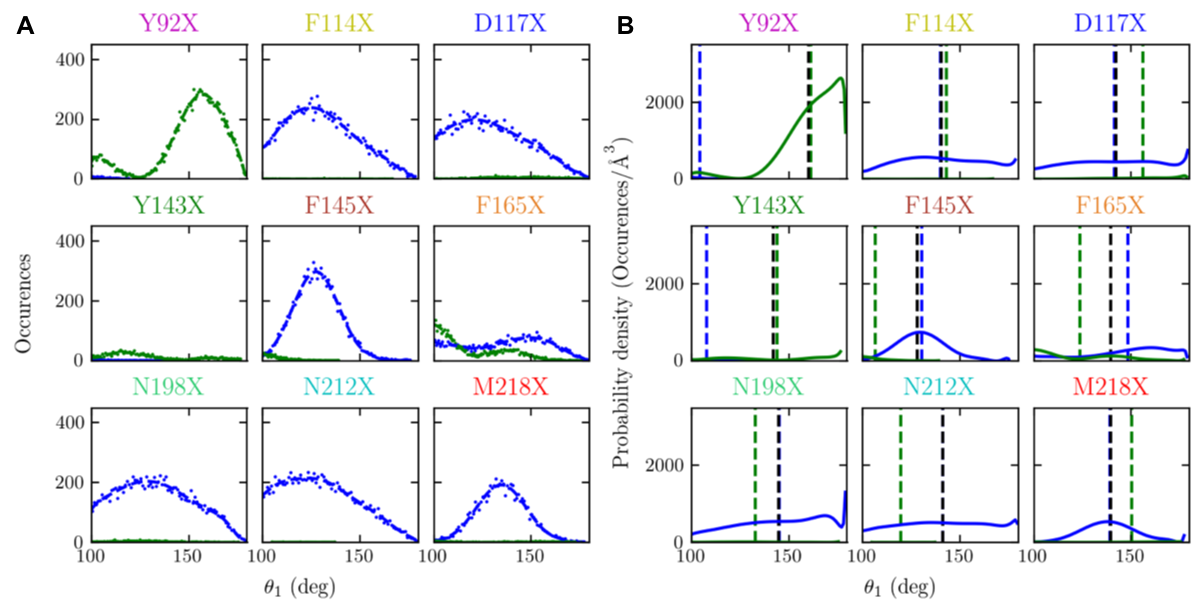
\includegraphics[width=\double]{figures-gfp-hbond/FigureS4_combined.png}
    \caption[Histograms of C--N$\cdots$H angle to calculate most probable $\theta_1$]{
        (A) A histogram of the C--N$\cdots$H angles ($\theta_1$) observed throughout the MD simulation for each nitrile location. 
        In blue are the angles observed of hydrogen bonding to water. 
        In green are the angles observed of hydrogen bonding to protein. 
        Each histogram (dots) was fit to a 10- term polynomial (solid lines) to remove the noise. 
        (B) The polynomial fits of the histograms were normalized by the volume element of each bin using Equation \ref{eq:angnorm} and are plotted. 
        The blue dashed line is the average angle of hydrogen bonds to water, green is the average angle of hydrogen bonds to protein, and black is the combined average angle of hydrogen bonding, where each average was taken from the normalized probabilities.
    }
    \label{fig:hbond-theta_histogram}
\end{figure}

For all nine probe locations investigated, we observed a strong correlation ($r = 0.944$) between the hydrogen bonding angle and the mean vibrational frequency, as Choi et al. predicted in their quantum mechanical calculations \cite{Choi2008}.
The strength of the correlation is somewhat surprising given the well-known inaccuracies of hydrogen bonding geometries in the Amber03 force field \cite{Paton2009}, and that we have not accounted for electrochromic effects contributing to the measured frequencies or for exchange-repulsion interaction-induced frequency shifts.
These two effects are expected to also influence the measured vibrational frequency.  

To account electrochromic effects that may contribute to the measured frequency, we estimated the extent of the Coulombic frequency shift by calculating the Coulombic field at the midpoint of the nitrile using a procedure described elsewhere \cite{Ensign2011}.
The calculated electric field is plotted against the mean vibrational frequency in Figure \ref{fig:hbond-forces}.
The calculated electric fields are poorly correlated to the mean vibrational frequency, suggesting that electrochromic effects play a minor role in contributing to the measured frequency.
We separately investigated the extent of the exchange-repulsion interaction-induced frequency shift in these systems by analyzing the hydrogen bond length parameter, $d_{\text{NH}}$.
The histograms and normalized probability densities for each hydrogen bonding distance bin are in Figure \ref{fig:hbond-hist_dist}, and the average distance is plotted against the mean vibrational frequency in Figure \ref{fig:hbond-abs_vs_dist}.
However, presumably because each of these distance interactions are governed by the same Lennard Jones potential from the Amber03 force field, the probability distributions of the lengths of hydrogen bonds to water are remarkably similar.
Thus, the average hydrogen bond distances are not well correlated to the experimental mean vibrational frequencies.
Because of the strong correlation of the hydrogen bonding angle, the lack of correlation of the calculated Coulombic field, and the lack of correlation of the average hydrogen bonding distance, we believe that the hydrogen bonding angle is the dominant contribution to the frequency in these cases.

\begin{figure}
    \center
    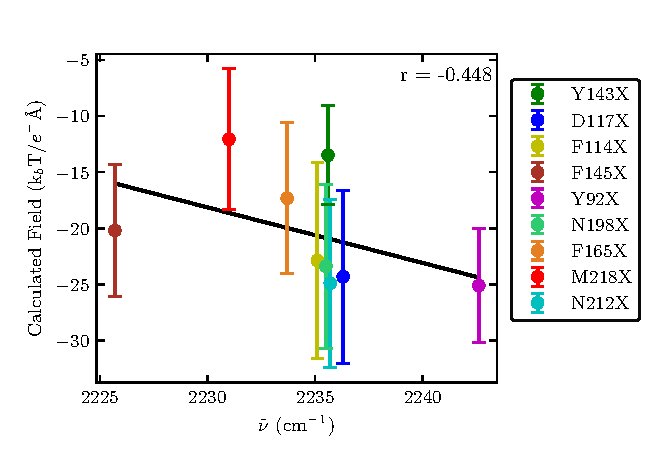
\includegraphics[width=\single]{figures-gfp-hbond/forces.pdf}
    \caption[Calculated forces compared to the experimental nitrile frequencies]{
        The Coulombic field was calculated at the midpoint of the nitrile for each frame in the 40 ns of production simulation. 
        The average Coulombic field ($y$-axis) is plotted against the experimental mean vibrational frequency ($x$-axis). 
        The error bars on the $y$-axis represent the standard deviation of the field. 
        All vibrational frequencies shown here were measured at 25 \si{\celsius}.
    }
    \label{fig:hbond-forces}
\end{figure}

\begin{figure}
    \center
    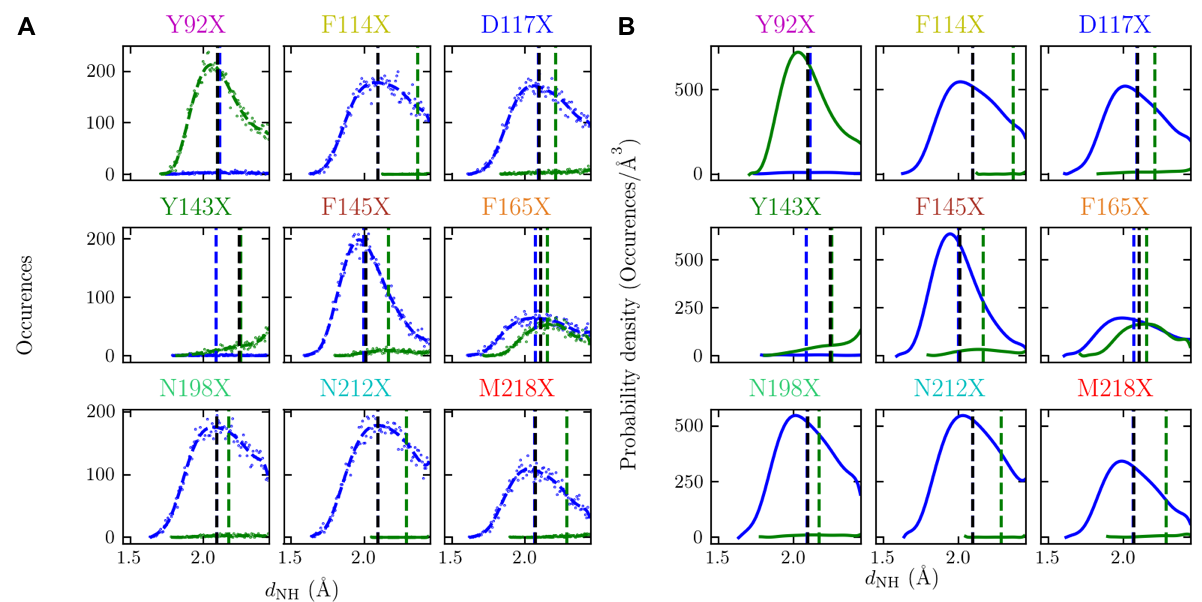
\includegraphics[width=\double]{figures-gfp-hbond/FigureS5_combined.png}
    \caption[Histograms of N--H lengths to calculate most probable $d_{\text{NH}}$]{
        (A) A histogram of the N--H lengths ($d_{\text{NH}}$) observed throughout the MD simulation for each nitrile location. 
        In blue are the hydrogen bonding lengths observed to water. 
        In green are the hydrogen bond lengths observed to protein. 
        Each histogram (dots) was fit to a 10-term polynomial (solid lines) to remove the noise. 
        (B) The polynomial fits of the histograms were normalized by the volume element of each bin and are plotted. 
        The blue dashed line is the average angle of hydrogen bonds to water, green is the average angle of hydrogen bonds to protein, and black is the combined average angle of hydrogen bonding, where each average was taken from the normalized probabilities. 
        Because the volume of the radial bins above are different than the angular bins, the volume element of each radial bin was computed with the equation: 
    $V = \frac{4\pi}{3}\left ( d_{\text{NH}}''^3 - d_{\text{NH}}'^3 \right )$, 
    where $V$ is the volume element of the bin and $d_{\text{NH}}'$ and $d_{\text{NH}}''$ are the bin edges of $d_{\text{NH}}$.
    }
    \label{fig:hbond-hist_dist}
\end{figure}

\begin{figure}
    \center
    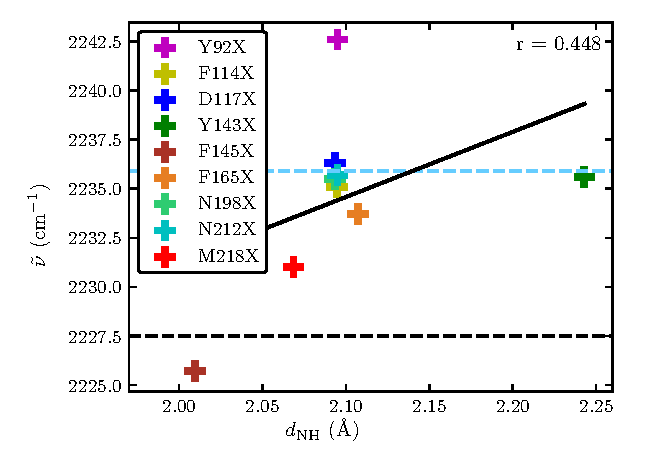
\includegraphics[width=\single]{figures-gfp-hbond/abs_max_vs_max_dist.pdf}
    \caption[Most probable $d_{\text{NH}}$ against experimental frequencies]{
        For each of the nine nitrile locations, the average distance of hydrogen bonding from simulation is plotted against the experimental mean vibrational frequency. 
        For reference, the mean vibrational frequency of the CNF in water is shown as a light-blue dashed line, and the mean vibrational frequency of \emph{p}-tolunitrile in THF is shown as a black dashed line. 
        All vibrational frequencies shown here were measured at 25 \si{\celsius}.
    }
    \label{fig:hbond-abs_vs_dist}
\end{figure}

In order to contribute to the line shape of the nitrile spectra, a given hydrogen bond would need to have a lifetime longer than the vibrational lifetime of the nitrile probe.
To determine whether or not that was the case for the hydrogen bond populations in Figure \ref{fig:hbond-heatmap}, we tracked each hydrogen bond in all nine trajectories.
As a function of simulation time, we plotted the number of hydrogen bonds that persisted for at least that length of time.
These plots were fit to an exponential decay function and are shown in Figure \ref{fig:hbond-lifetimes}.
The lifetimes were calculated from the decay rate and are reported in Table \ref{tbl:hbond-lifetimes}.
All but one hydrogen bonding population had a lifetime approximately equal to or longer than the vibrational lifetime of CNF, which is estimated to be on the order of a picosecond or less \cite{Ghosh2009, Ha2009, Waegele2010}, suggesting that these populations contribute to the line shape of the nitrile absorption spectrum.

\begin{figure}
    \center
    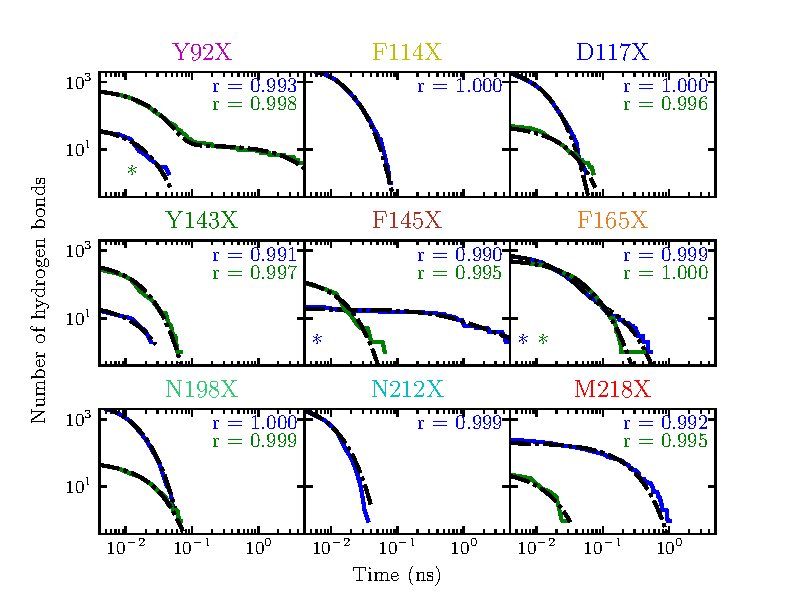
\includegraphics[width=\double]{figures-gfp-hbond/Lifetime_hbonds.pdf}
    \caption[Residence lifetimes of observed hydrogen bonds]{
        For every hydrogen bond in each simulation, the lifetime of the hydrogen bond (simulation time elapsed before the interaction is no longer classified as a hydrogen bond) was calculated. 
        These lifetimes are plotted against simulation time where the $y$-axis is the number of hydrogen bonds observed that lasted \emph{at least} as long as the simulation time, the $x$-axis. 
        In blue, the lifetimes of hydrogen bonds to water are shown. 
        In green, the lifetimes of hydrogen bonds to protein are shown. 
        The black dashed lines are exponential decay fits, with $r$-values displayed in the upper-right corner. 
        A star indicates that two hydrogen populations were observed with significantly different decay rates. 
        These cases were fit to a double exponential decay.
    }
    \label{fig:hbond-lifetimes}
\end{figure}

\begin{table}
    \caption[Estimated lifetimes of hydrogen bonding interactions]{
        The lifetime of each hydrogen bonding population fit with an exponential decay in Figure \ref{fig:hbond-lifetimes}. 
        For nitriles that were observed to have two hydrogen bonding populations with significantly decay rates, a double exponential was fit to the data, and therefore two lifetimes are reported.
    }
    \begin{center}
    \begin{tabular}{r | c c | c c}
    & \multicolumn{2}{c}{Water} & \multicolumn{2}{c}{Protein}\\
    \toprule
        Mutant &  $\tau_1$ (ps)  & $\tau_2$ (ps) &  $\tau_1$ (ps) & $\tau_2$ (ps) \\
    \midrule
    
        Y143X & 10.3  &        & 9.7   &          \\
        D117X & 6.6   &        & 17.9  &          \\
        F114X & 9.3   &        & 15.7  &          \\
        F145X & 653.8 & 5228.8 & 8.3   &          \\
        Y92X  & 11.1  &        & 17.0  & 3095.7   \\
        N198X & 7.3   &        & 15.1  &          \\
        F165X & 15.2  & 112.2  & 23.7  & 44.7     \\
        M218X & 149.2 &        & 9.0   &          \\
        N212X & 5.5   &        & 0.5   &          \\
    
    
    \bottomrule
    \end{tabular}
    \end{center}
    \label{tbl:hbond-lifetimes}
\end{table}

It is interesting to note that out of all of our nine protein systems, not a single nitrile location was free from hydrogen bonding.
While this certainly may be an artifact of GFP with its unique water filled \textbeta{}-barrel structure, it appears that hydrogen bonding to the nitrile is so favorable that even when placed in a location with no solvent accessibility, the nitrile will find a donor other than water.
For example, when we put the nitrile at position 92, a location with virtually no solvent exposure, we observed that the nitrile was involved in significant hydrogen bonding with protein atoms.
Additionally, when we put the nitrile at position 143, a location that was void of any conventional hydrogen bond donors, the nitrile experienced transient hydrogen bonds from an electron poor carbon atom.
The observation of these weak hydrogen bonds from carbon suggests that even if there are no strong hydrogen bond donors nearby, the nitrile will still engage in interactions to fulfill its hydrogen bond accepting capabilities.
If these observations of nitrile-labeled GFP extend to other systems, this would certainly complicate the interpretation of nitrile spectra in biological systems.
Our results suggest that, to properly interpret nitrile spectra, one must \emph{always} consider hydrogen bonding effects.
Because of the consistent presence of hydrogen bonds and the strong correlation between the hydrogen bonding angle and the mean vibrational frequency, it is necessary to determine the geometry of hydrogen bonds to the nitrile in all reference and perturbed states to ensure that the measured frequency shifts are not due to change in hydrogen bond geometry.
A constant frequency offset, such as the 10 \si{\wn} offset suggested by Fafarman et al. \cite{Fafarman2010}, cannot be applied to nitrile frequencies in protein systems where the hydrogen bonding orientation is easily constrained by the protein surroundings, such as an enzyme active site or in the interior of a protein.
Specifically, when measuring a particular perturbation via vibrational spectroscopy of a nitrile, the FTLS of the reference and perturbed state may be used to confirm that specific hydrogen bonding interactions do not change substantially between the two states.

Certainly, we have shown that a Boolean classification of the existence of hydrogen bonding is insufficient when the nitrile is placed in complex protein environments.
There is a broad range of hydrogen bonding interactions available to a nitrile probe, and each circumstance contributes differently to the nitrile frequency.
This means that there is not a constant change in frequency that can universally be applied to all hydrogen bonding interactions.
However, the ability of nitriles to accept hydrogen bonds should not be interpreted as a disadvantage for its use as a vibrational probe.
The strength of the correlation in Figure \ref{fig:hbond-comparison}B demonstrates that is possible to decouple the hydrogen bonding shift from other spectroscopic effects, such as the VSE, when there is sufficient molecular information about the hydrogen bonding geometry and FTLS.

%%%%%%%%%%%%%%%%%%%%%%%%%%%%%%%%%%%%%%%%%%%%%%%%%%%%%%%%%%%%%%%%
%%%%%%%%%%%%%%%%%%%%%%%%%%%%%%%%%%%%%%%%%%%%%%%%%%%%%%%%%%%%%%%%
\section{Conclusions}\index{hbond-conclusion}
%%%%%%%%%%%%%%%%%%%%%%%%%%%%%%%%%%%%%%%%%%%%%%%%%%%%%%%%%%%%%%%%
%%%%%%%%%%%%%%%%%%%%%%%%%%%%%%%%%%%%%%%%%%%%%%%%%%%%%%%%%%%%%%%%

We have experimentally measured the temperature-dependent frequencies of CNF in nine different locations across the GFP protein and demonstrated the broad range of hydrogen bonding environments present in a complex protein system.
We showed that the FTLS is directly related to molecular level details of the specific hydrogen bonding interactions to the nitrile probe.
The FTLS is strongly correlated to the SASA of the CNF probe, except in cases where constrained molecular geometry resulted in significant hydrogen bonding that was not captured by SASA.
Nevertheless, it appears the FTLS of a nitrile probe can be used to rapidly assess the degree of hydrogen bonding of the nitrile, even in the dynamic and complex environment found in and around a protein.
These molecular-level details are essential for properly interpreting the vibrational spectrum of the nitrile probe in any experiment where the specific hydrogen bonding interactions may be changing.
This is especially necessary to ensure that a VSE experiment is actually reporting on a change in electric field instead of reflecting sensitivity to subtle changes in hydrogen bonding geometries. 

We have further demonstrated the significant effect of hydrogen bonding on the nitrile spectra by showing that in our nine CNF containing variants, the mean nitrile vibrational frequency was dominated by the hydrogen bonding geometry, and that the measured frequencies matched what was expected from a theoretical prediction of the effect of hydrogen bonding geometry on nitrile frequency.
In every one of our systems, the CNF probe experienced some type of hydrogen bonding.
For all observed variants, the average hydrogen bonding angle was well correlated with the mean vibrational frequency observed in experiment.
Additionally, the fwhm of the experimental spectra were qualitatively consistent with the distribution of the hydrogen bonding geometries from simulation.
Finally, we have shown that FTLS measurements may be used to assess the hydrogen bonding interactions of a nitrile so that they may be properly accounted for in the interpretation of the spectra.





